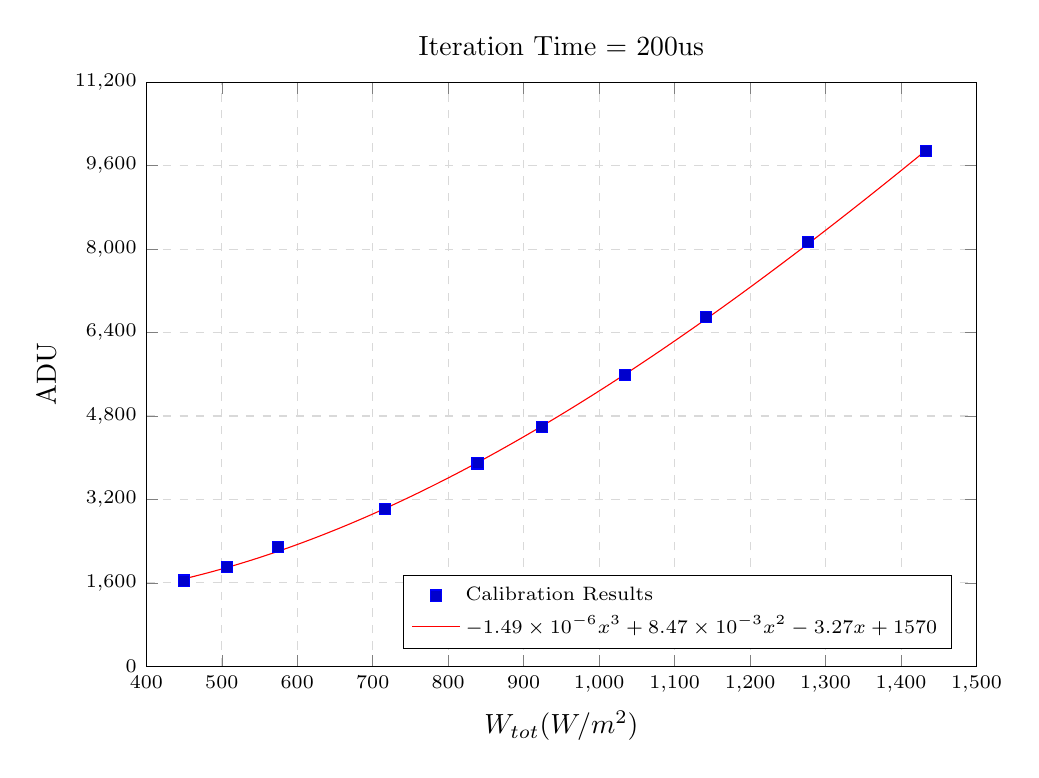
\begin{tikzpicture}
\begin{axis}[
	title = {Iteration Time = 200us},
    tick label style={font=\scriptsize},
    legend style={font=\scriptsize,/tikz/column 2/.style={column sep=5pt},},
    %legend columns=2,
    legend cell align=left,
	legend pos =south east,
    grid=major, % Display a grid
    grid style={dashed,gray!30}, % Set the style
    xlabel={$W_{tot} (W/m^2)$},
    ylabel={ADU}, 
    ymin = 0, ymax = 11200,
    %ytick={300,325,350,375,400,425,450,475,500,525},
    %yticklabels={300,325,350,375,400,425,450,475,500,525},
    xmin = 400, xmax = 1500,
    ytick={0,1600,...,11200},
    yticklabel style={
        /pgf/number format/fixed,
        /pgf/number format/precision=5},
	scaled y ticks=false,
    width=\textwidth, height=9cm,
    ]
\addplot+[only marks,mark=square*,blue]
coordinates {(	449.9120215	,	1645	)
(	506.9481463	,	1900	)
(	574.5844207	,	2285	)
(	716.4103256	,	3021	)
(	838.8604805	,	3890	)
(	924.4022127	,	4596	)
(	1034.669156	,	5586	)
(	1141.371929	,	6690	)
(	1276.958202	,	8139	)
(	1433.317083	,	9885	)
};
\addlegendentry{Calibration Results}
\addplot[
    domain=450:1430, 
    samples=100, 
    color=red,
]{0.00847*x^2 - 0.00000149*x^3 - 3.27*x + 1570};
\addlegendentry{$-1.49\times 10^{-6}x^3 + 8.47\times 10^{-3}x^2 - 3.27x + 1570$}
\end{axis}
\end{tikzpicture}